\maketitle

\section{Introduction}

\begin{frame}[fragile]{Motivation}
\centering
\only<1>{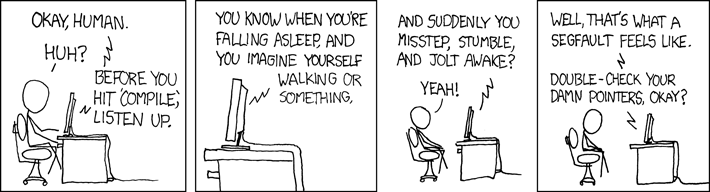
\includegraphics[width=\textwidth]{img/compiler_complaint.png}}

\only<2>{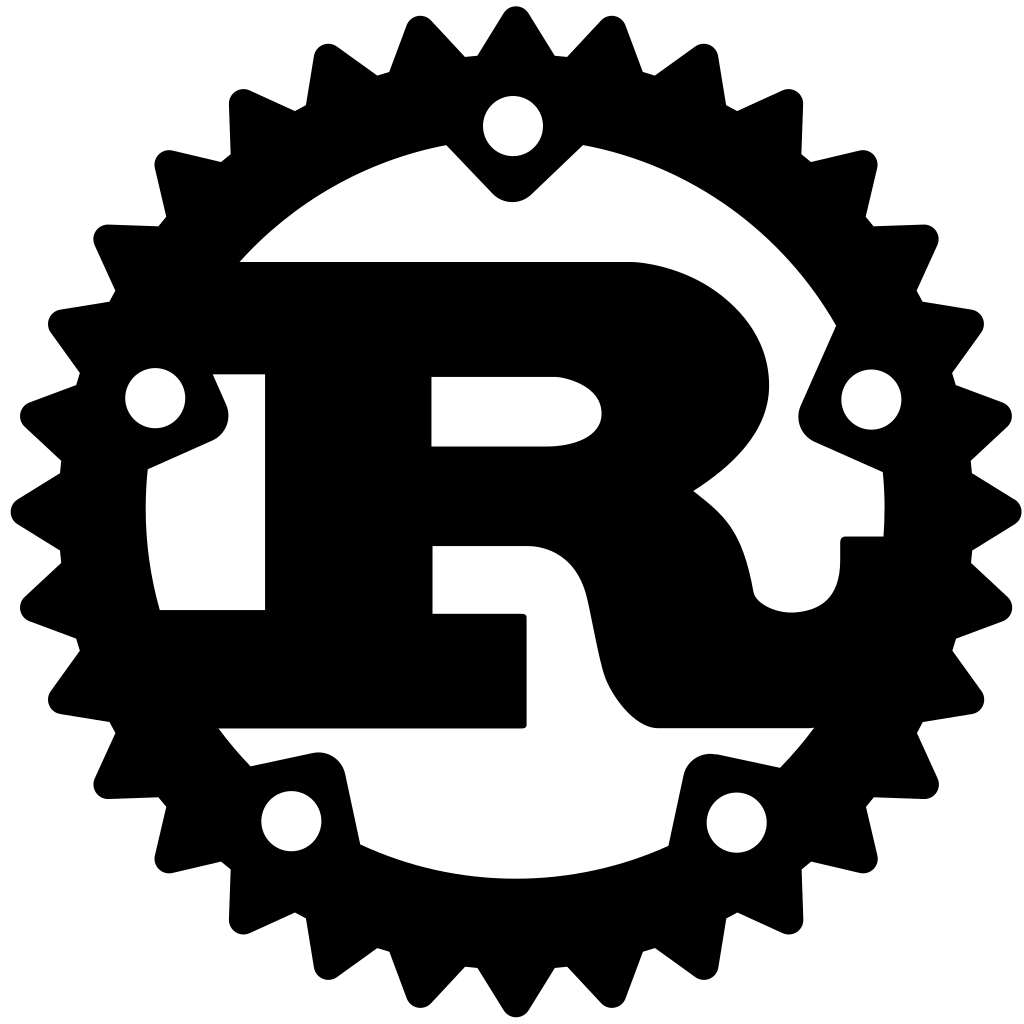
\includegraphics[width=0.3\textwidth]{img/rust.png}}

\begin{onlyenv}<3>
\begin{lstlisting}[style=short, language=Rust]
/// Returns the square of `x`. Squares are non-negative.
fn square(x: i32) -> i32 { -2 * x }
\end{lstlisting}
\end{onlyenv}
\begin{onlyenv}<4>
\begin{lstlisting}[style=short, language=Rust]
/// Returns the square of `x`. Squares are non-negative.
#[post(ret >= 0)]
fn square(x: i32) -> i32 { -2 * x }
\end{lstlisting}
\end{onlyenv}
\begin{onlyenv}<5>
\begin{lstlisting}[style=short]
- Result for 'postcondition' VC for square @?:?:
-2 * x >= 0
=> INVALID
Found counter-example:
 x: Int -> 1
\end{lstlisting}
\end{onlyenv}
\end{frame}


\begin{frame}{Presenting our tool}
  \begin{columns}
  \column{0.5\textwidth}
  \centering
  \Large{\texttt{rust-stainless}}

  \column{0.5\textwidth}
  \centering
  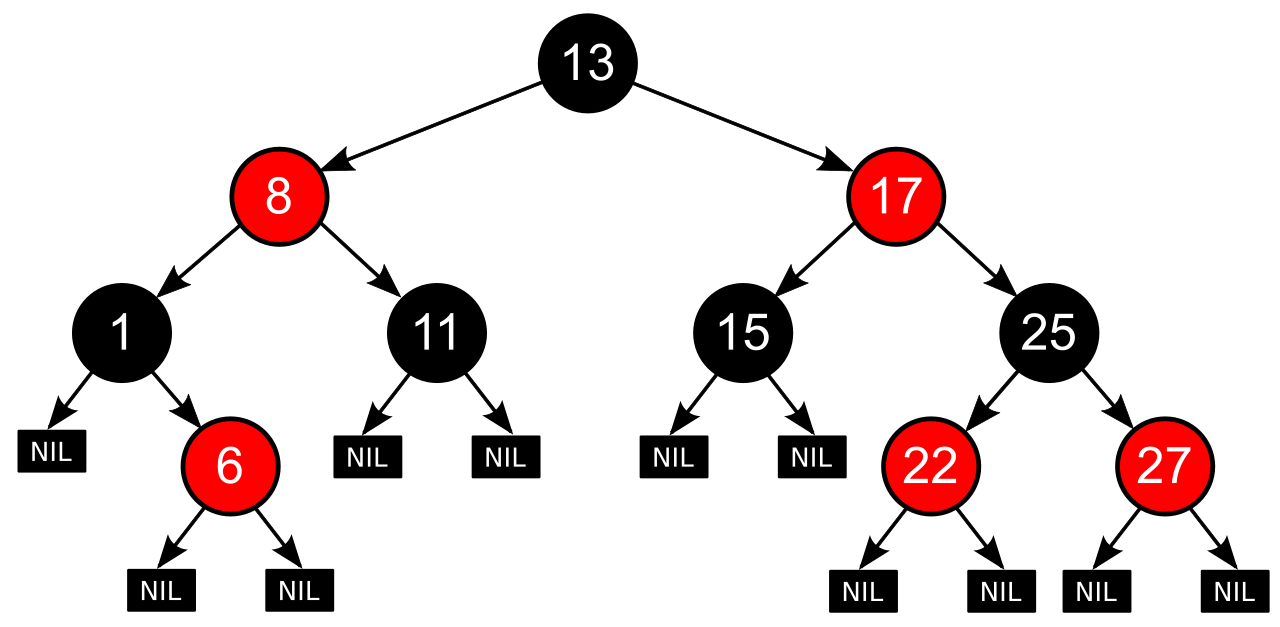
\includegraphics[width=\textwidth]{img/rbtree.png}
\end{columns}
\end{frame}


\begin{frame}{Contents}
  \setbeamertemplate{section in toc}[sections numbered]

  \tableofcontents%[hideallsubsections]

  \textit{Keeping it specific.}
\end{frame}

\section{Verifying a Red-Black Tree}

\begin{frame}{Red-Black Tree}
\begin{columns}[T]
\column{0.5\textwidth}
\begin{itemize}
  \item Binary search tree
  \item Lookup, insertion and deletion in $\mathcal{O}(\log n)$ time
  \only<2->{  \item But only if well balanced }
  \only<3->{
    \item Red-Black Tree uses colouring to automatically rebalance at insertion
    and deletion
  }
\end{itemize}

\column{0.5\textwidth}
\centering
\only<1>{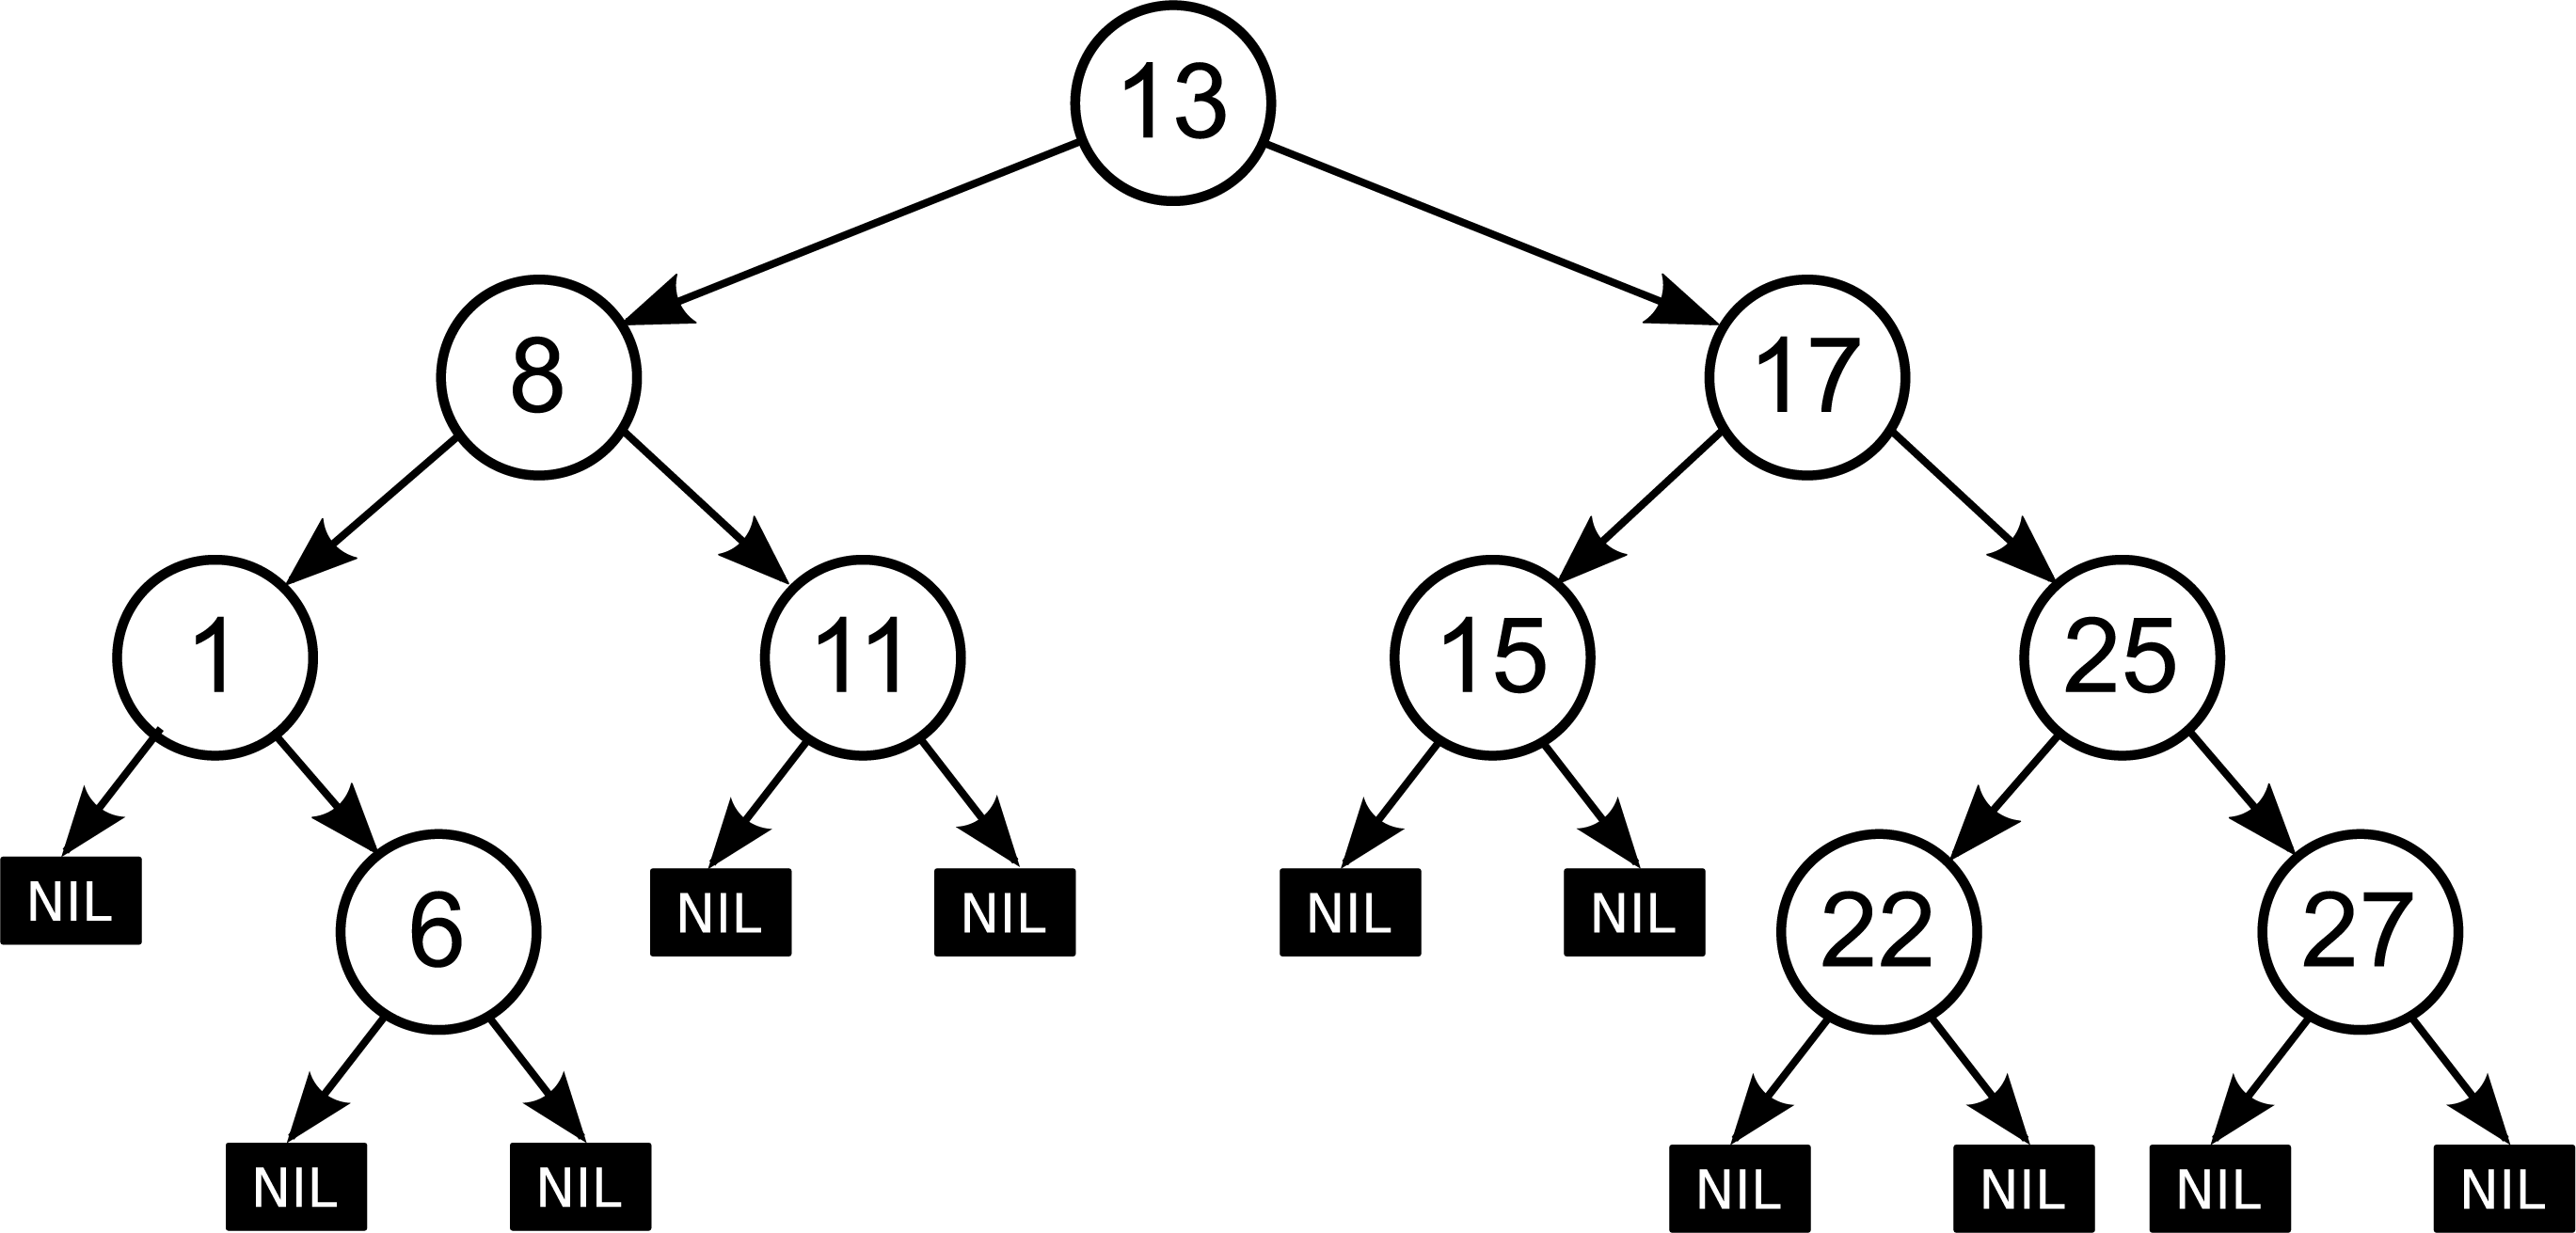
\includegraphics[width=\textwidth]{img/binary_tree.png}}
\only<2>{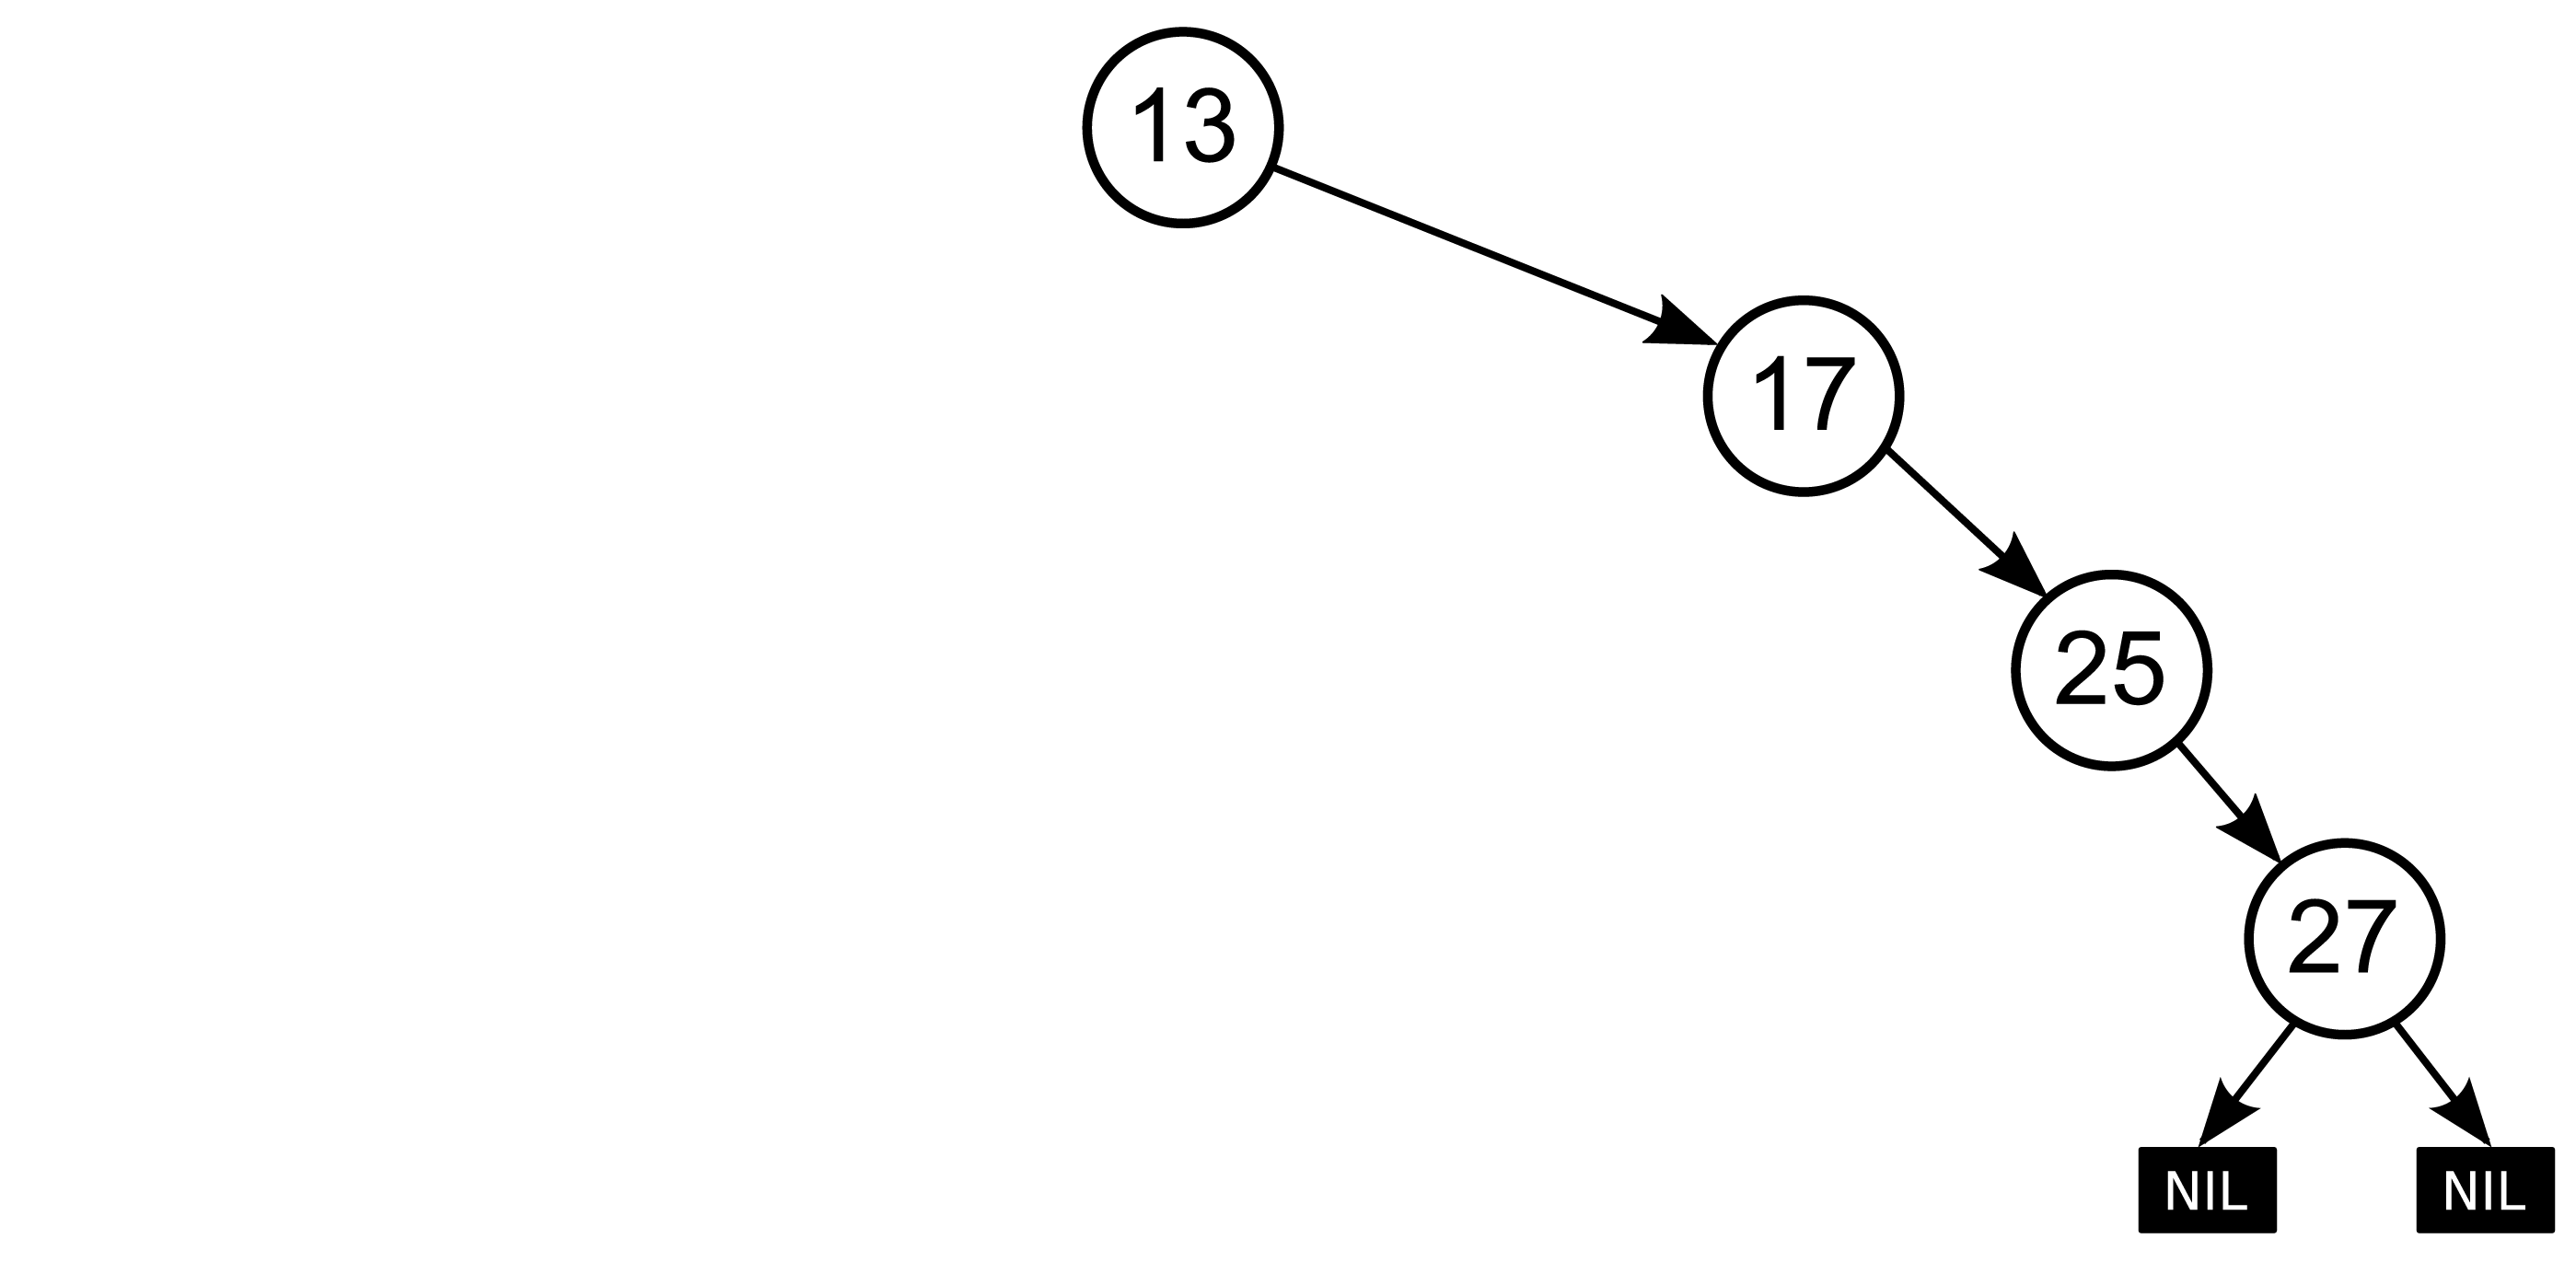
\includegraphics[width=\textwidth]{img/binary_tree_unbalanced.png}}
\only<3>{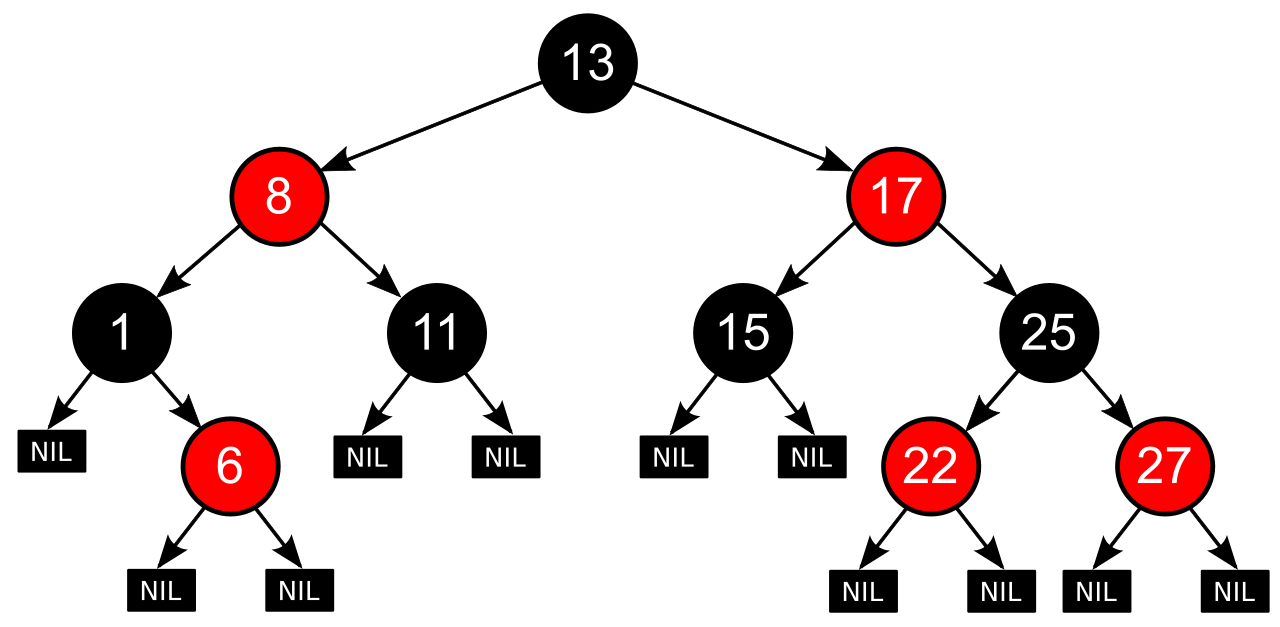
\includegraphics[width=\textwidth]{img/rbtree.png}}
\end{columns}
\end{frame}

\begin{frame}[standout]
  Why verify it?
\end{frame}

\begin{frame}{Red-Black Tree}
\textbf{Properties} \cite{rbtree}
\begin{columns}[T]
\column{0.5\textwidth}
\begin{enumerate}
  \item Each node is either red or black.
  \item All NIL (empty) nodes are considered black.
  \item A red node does not have a red child.
  \item Every path from a given node to any of its descendant NIL nodes goes through the same number of black nodes.
  \item (The root is black.)
\end{enumerate}

\column{0.5\textwidth}
\centering
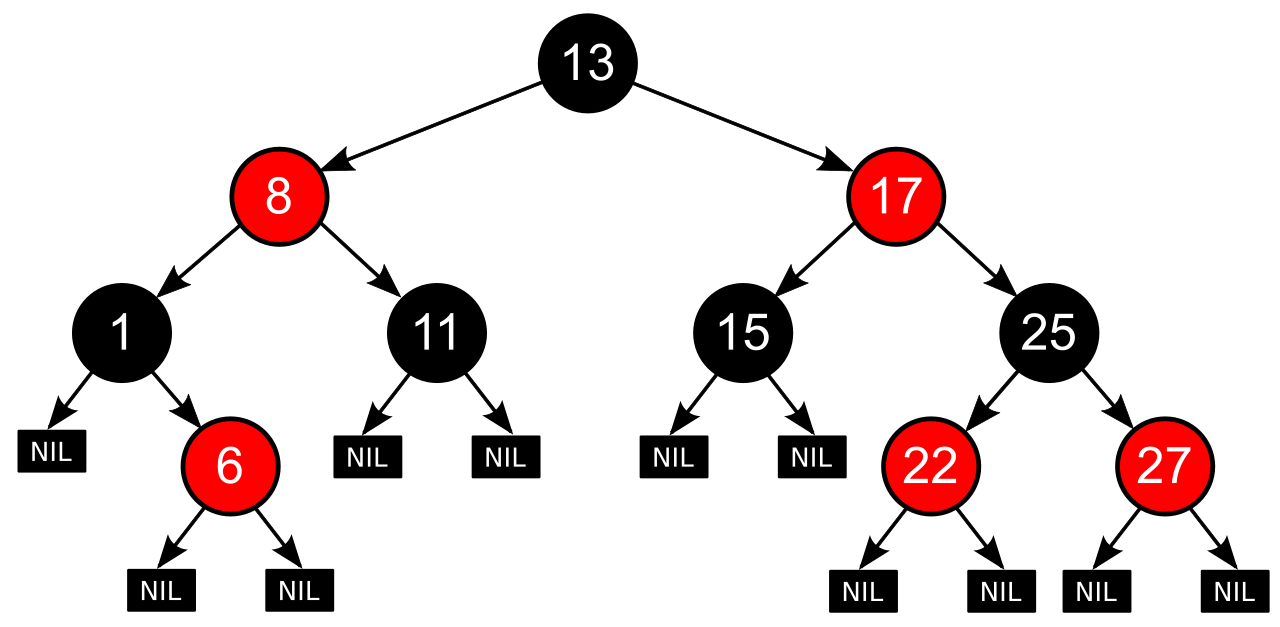
\includegraphics[width=\textwidth]{img/rbtree.png}
\end{columns}
\end{frame}

\begin{frame}{Insertion}
\begin{columns}[T]
\column{0.5\textwidth}
\textbf{Algorithm}
\begin{enumerate}
  \item Recursively descend in tree to correct position
  \only<2>{
    \item Insert a new red node
    \item Recursively go back up and solve all property violations
  }
\end{enumerate}

\column{0.5\textwidth}
\centering
\only<1>{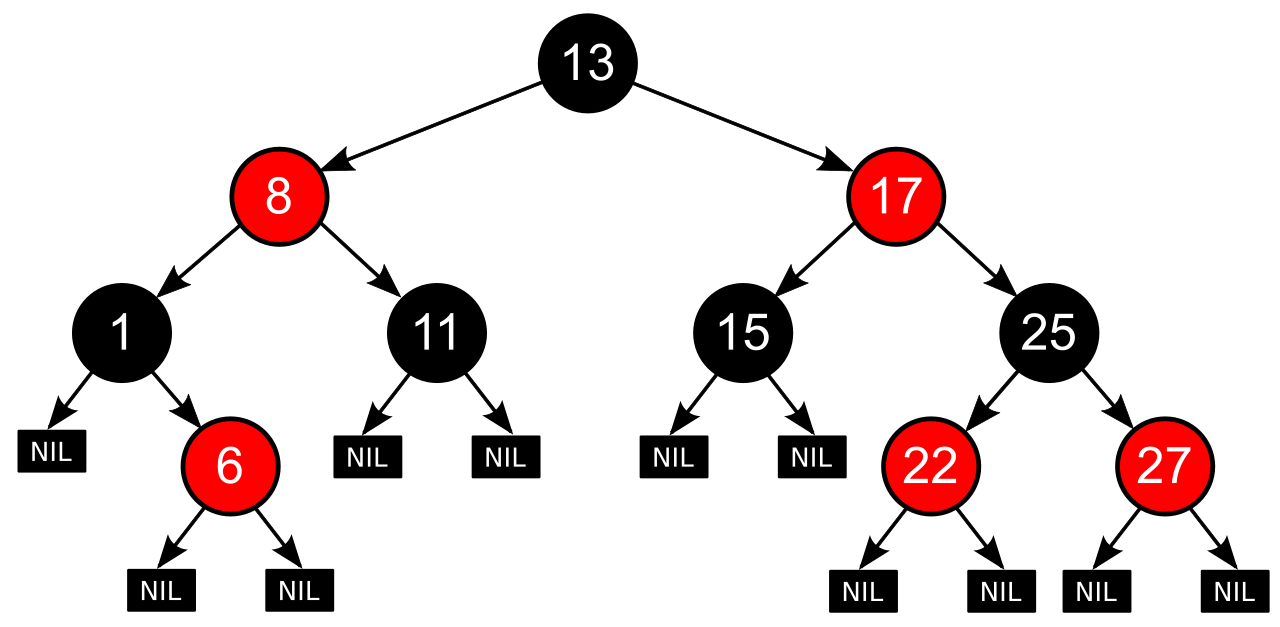
\includegraphics[width=\textwidth]{img/rbtree.png}}
\only<2>{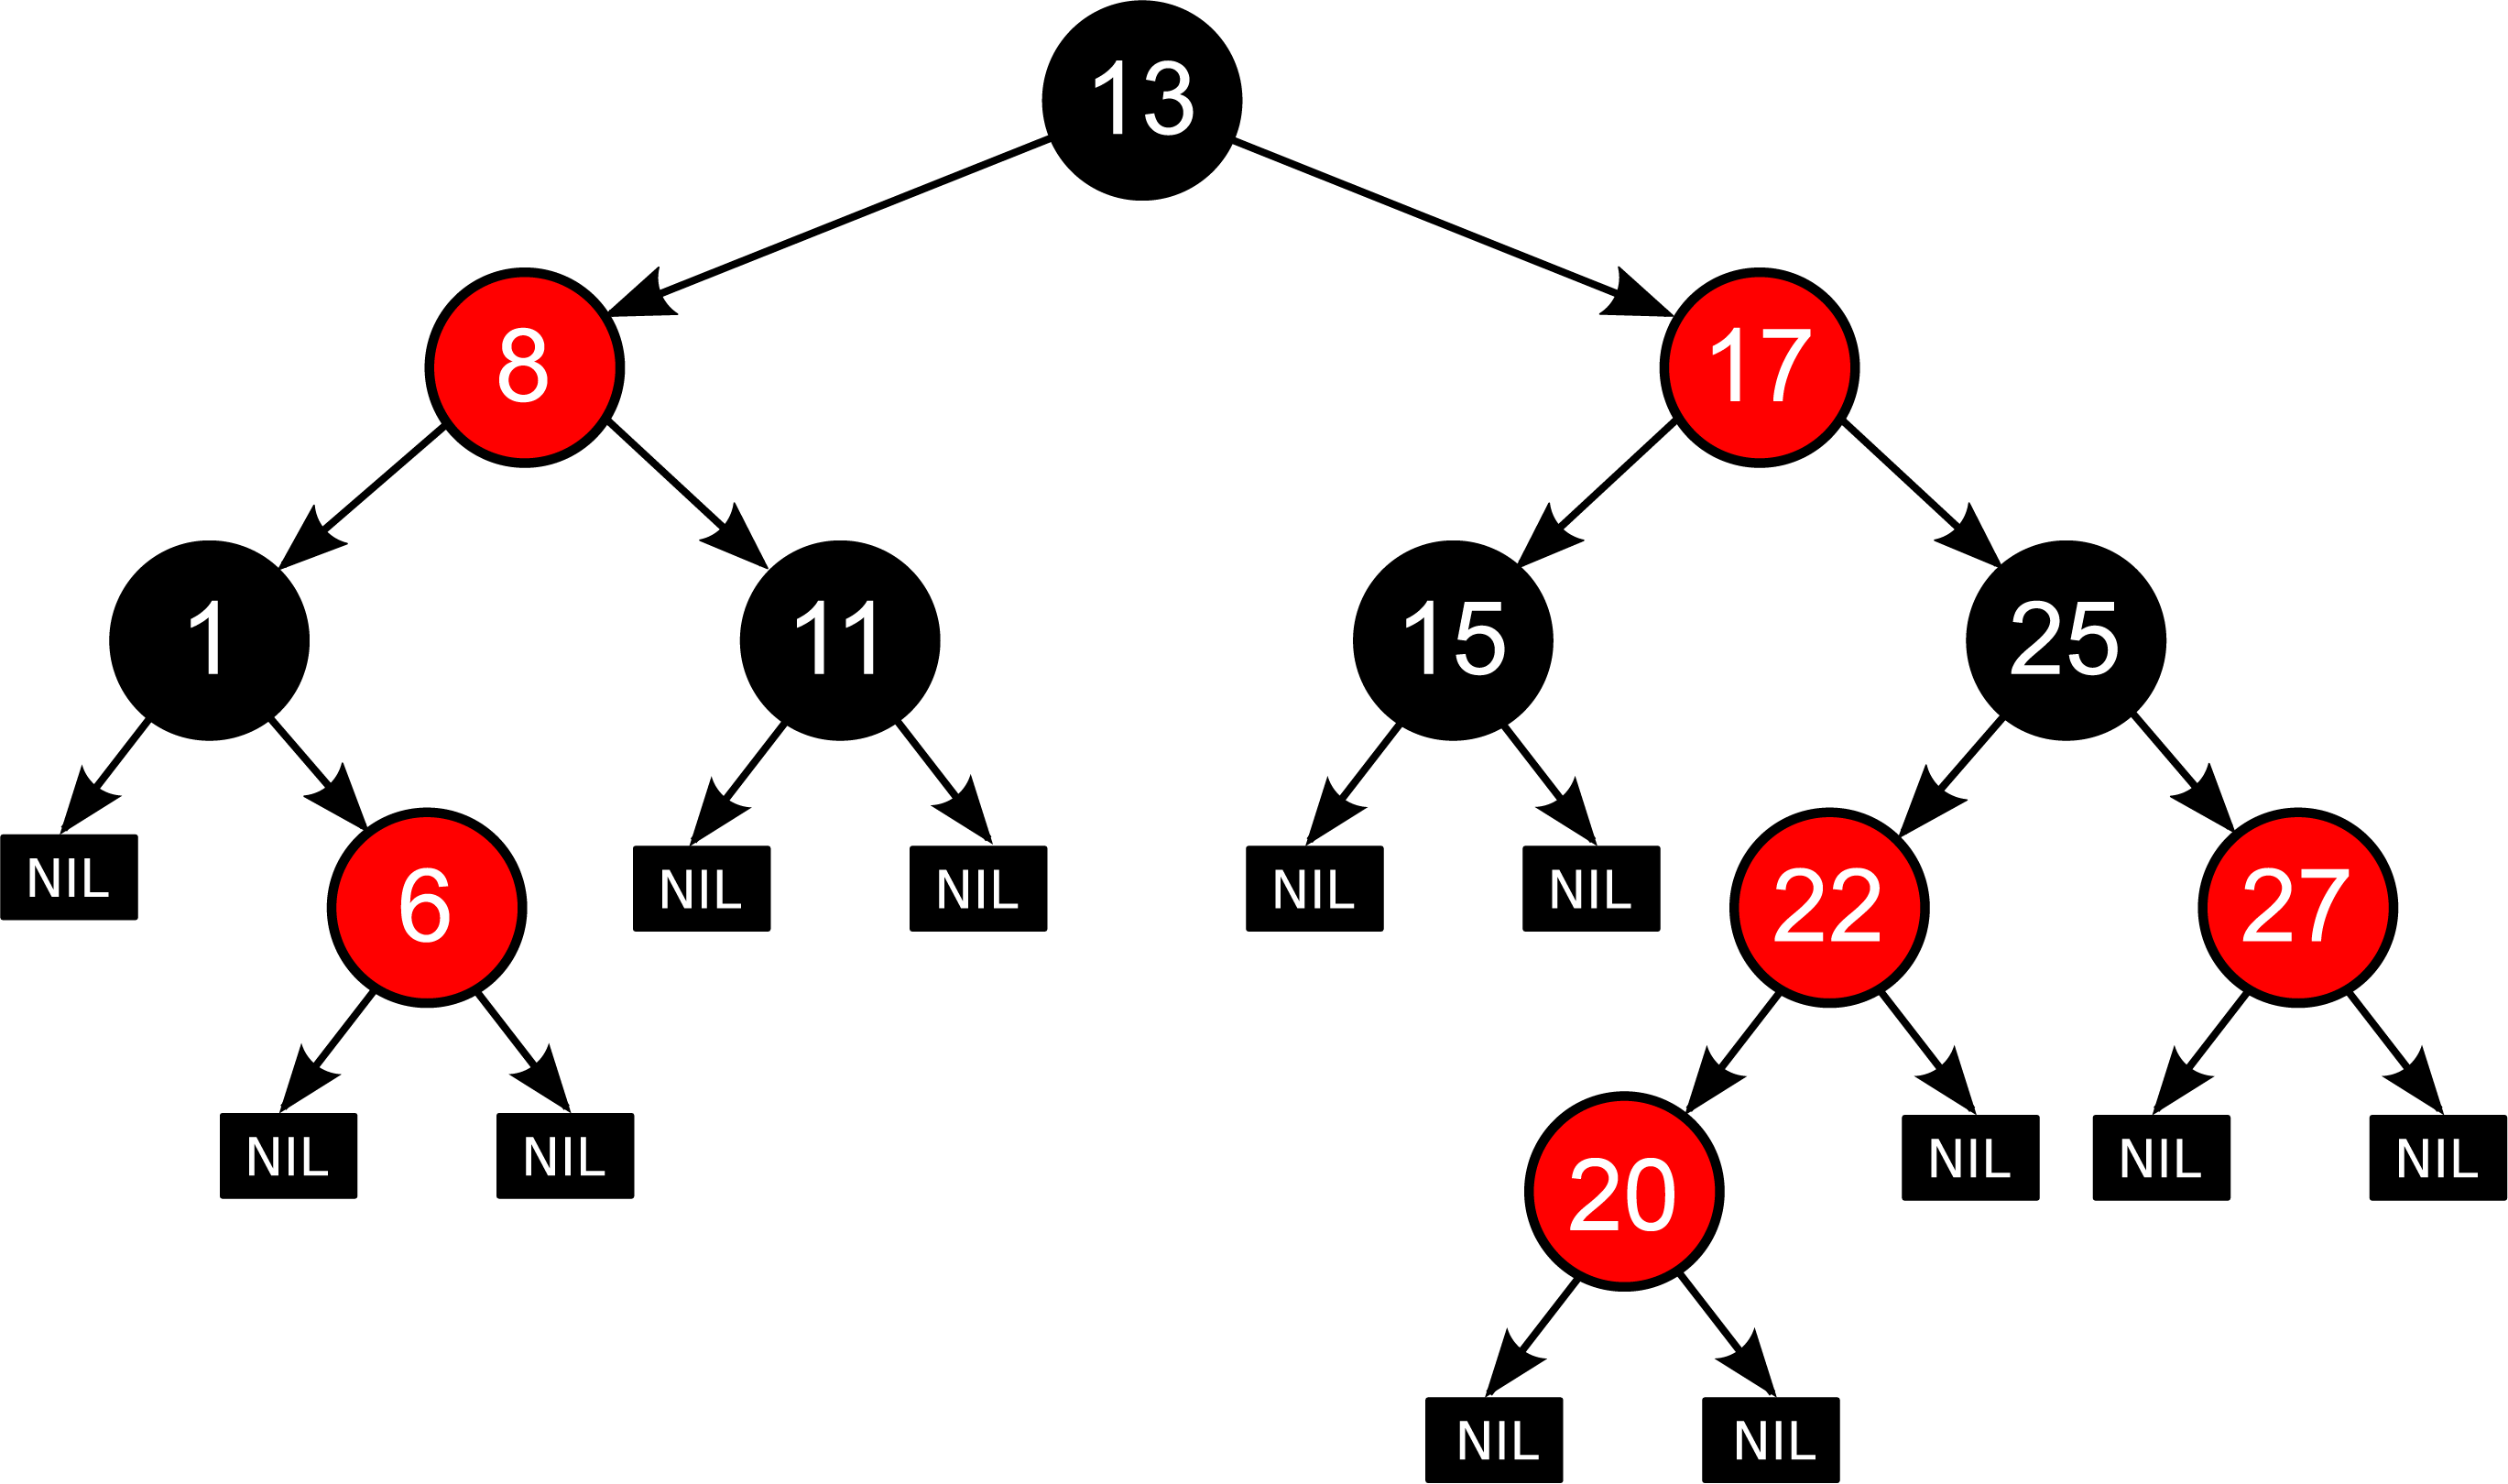
\includegraphics[width=\textwidth]{img/rbtree_insert.png}}
\end{columns}
\end{frame}

\begin{frame}[fragile]{Insertion}
In Scala
\begin{lstlisting}[language=Scala, basicstyle=\footnotesize\ttfamily]
def ins(x: BigInt, t: Tree): Tree = {
  require(redNodesHaveBlackChildren(t) && blackBalanced(t))
  t match {
    case Empty() => Node(Red(),Empty(),x,Empty())
    case Node(c,a,y,b) =>
      if      (x < y)  balance(c, ins(x, a), y, b)
      else if (x == y) Node(c,a,y,b)
      else             balance(c,a,y,ins(x, b))
  }
} ensuring (res => content(res) == content(t) ++ Set(x)
                 && size(t) <= size(res) && size(res) <= size(t) + 1
                 && redDescHaveBlackChildren(res)
                 && blackBalanced(res))
\end{lstlisting}
\end{frame}

\begin{frame}[fragile]{Rebalancing}
In Scala
\begin{lstlisting}[language=Scala, basicstyle=\footnotesize\ttfamily,]
def balance(c: Color, a: Tree, x: BigInt, b: Tree): Tree = {
    Node(c,a,x,b) match {
      case Node(Black(),Node(Red(),Node(Red(),a,xV,b),yV,c),zV,d) =>
        Node(Red(),Node(Black(),a,xV,b),yV,Node(Black(),c,zV,d))
      case Node(Black(),Node(Red(),a,xV,Node(Red(),b,yV,c)),zV,d) =>
        Node(Red(),Node(Black(),a,xV,b),yV,Node(Black(),c,zV,d))
      case Node(Black(),a,xV,Node(Red(),Node(Red(),b,yV,c),zV,d)) =>
        Node(Red(),Node(Black(),a,xV,b),yV,Node(Black(),c,zV,d))
      case Node(Black(),a,xV,Node(Red(),b,yV,Node(Red(),c,zV,d))) =>
        Node(Red(),Node(Black(),a,xV,b),yV,Node(Black(),c,zV,d))
      case Node(c,a,xV,b) => Node(c,a,xV,b)
    }
  } ensuring (res => content(res) == content(Node(c,a,x,b)))
\end{lstlisting}
\end{frame}

\begin{frame}{Rebalancing}
  \centering
  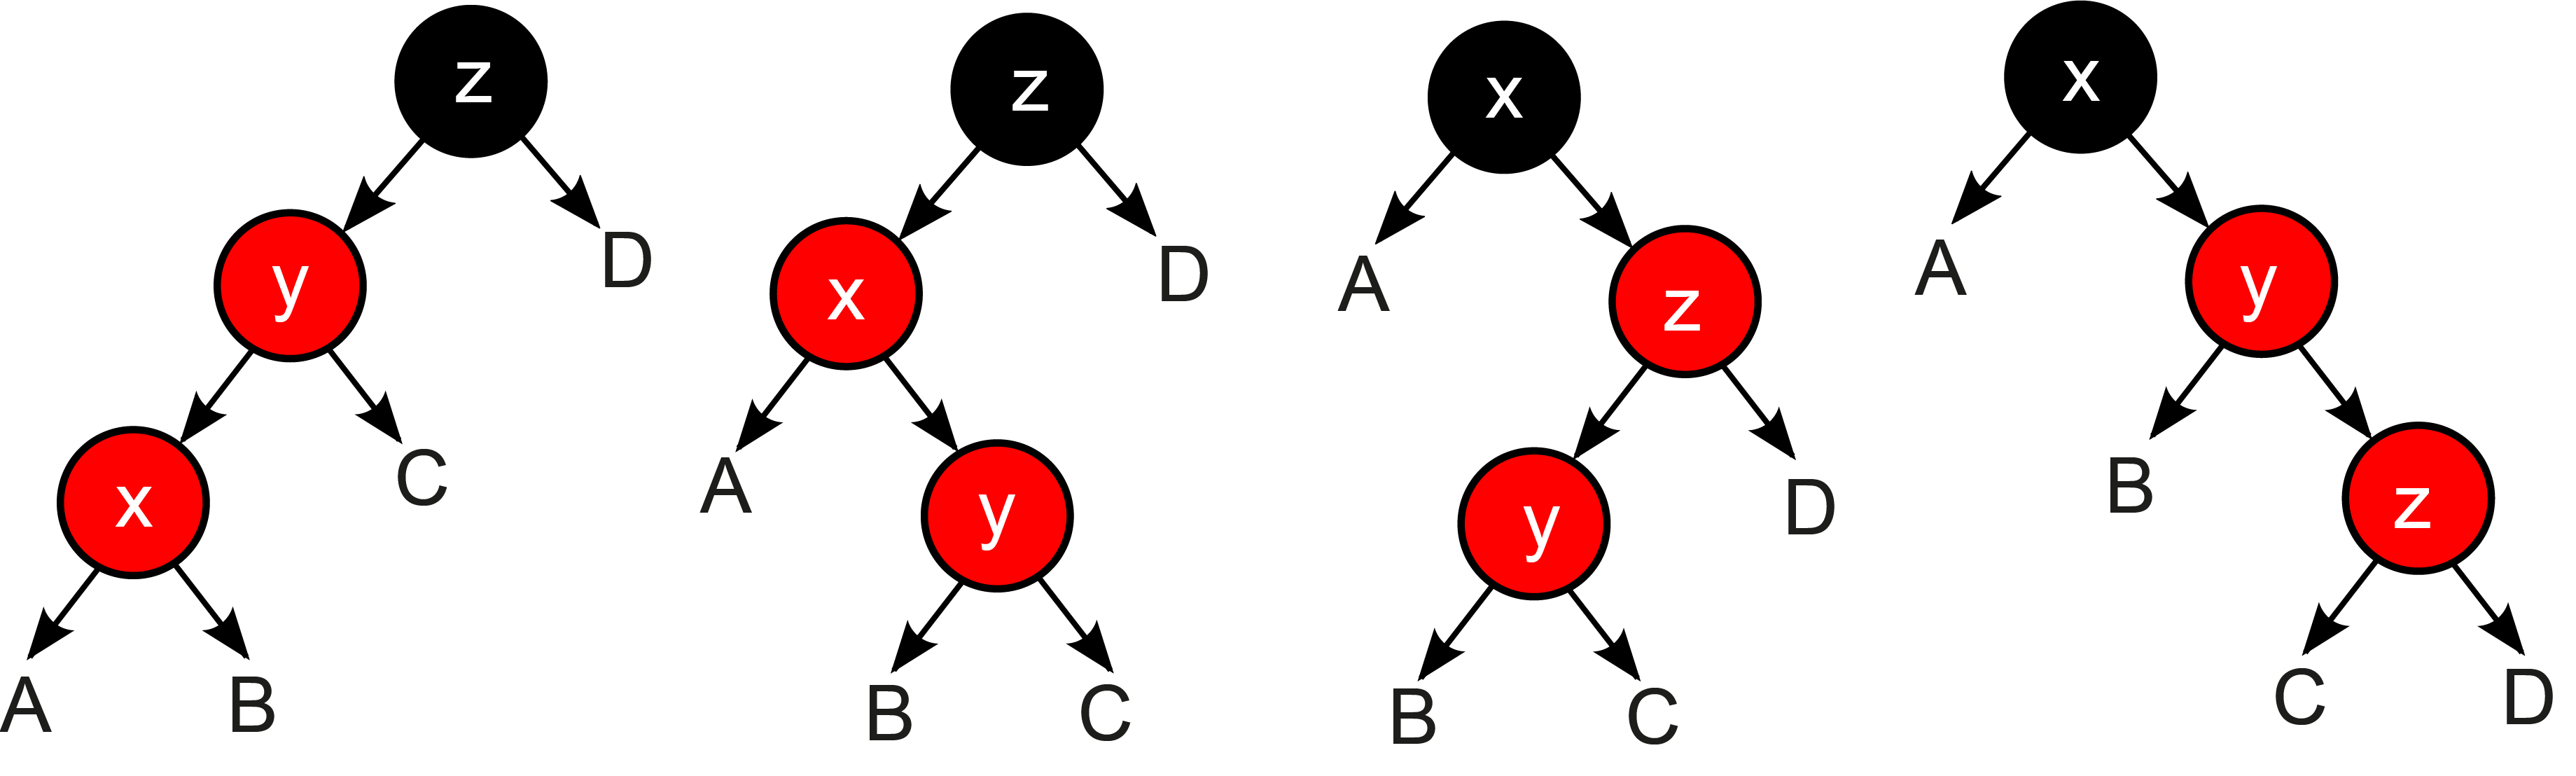
\includegraphics[width=0.8\textwidth]{img/rbtree_cases.png}
  \vfill
  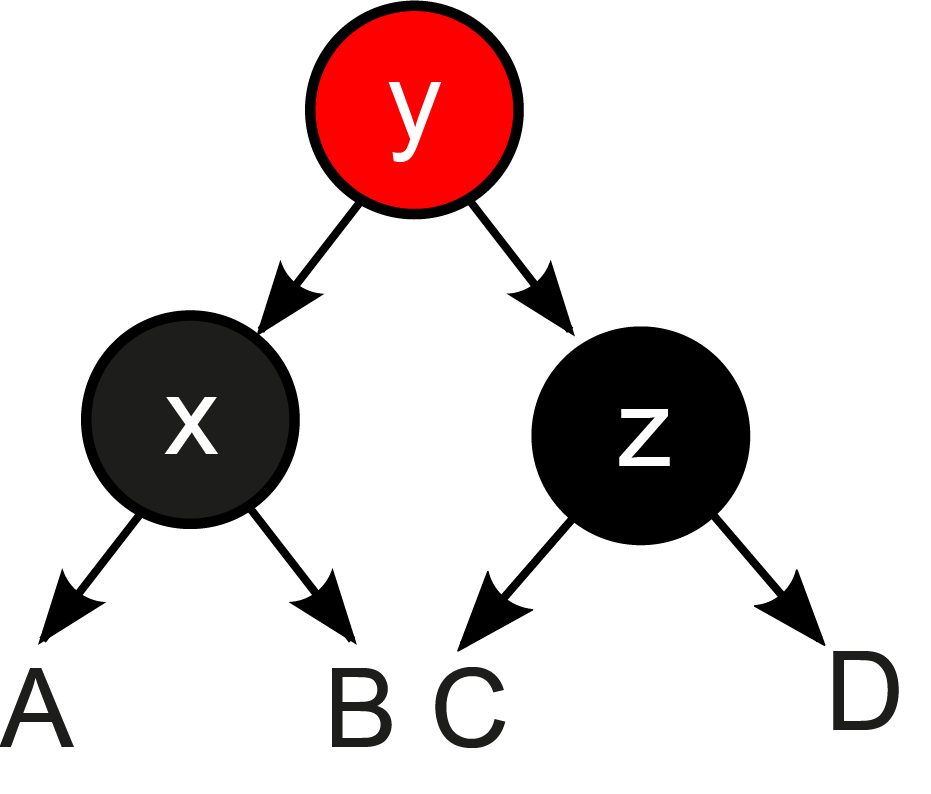
\includegraphics[width=0.3\textwidth]{img/rbtree_solution.png}
\end{frame}

\begin{frame}[standout]
  Why in Rust?
\end{frame}

\begin{frame}{Performance Comparison}
To insert the integers from 1 to 5000 into the implementation takes:
\begin{itemize}
  \item Red-Black Tree in Scala, fully functional, no mutation: 185s
  \only<2>{
    \item  Red-Black Tree in Rust, fully mutable, no allocation
    in rebalancing: \textbf{10ms}
  }
\end{itemize}
\end{frame}

\begin{frame}[fragile]{Red-Black Tree in Rust}
\begin{lstlisting}[language=Rust, caption={Data types with heap allocation}]
enum Color {
  Red,
  Black,
}

enum RBTree<T> {
  Empty,
  Node(Color, Box<RBTree<T>>, T, Box<RBTree<T>>),
}
\end{lstlisting}
\end{frame}


\begin{frame}[fragile]{Red-Black Tree in Rust}
\begin{lstlisting}[language=Rust, caption={Insert method with specification}]
impl RBTree<i32> {
  #[pre(
    self.red_nodes_have_black_children()
    && self.black_balanced()
  )]
  #[post(set_equals(
      &self.content(),&old(&self).content().insert(&t)
    ) && (old(&self).size() == self.size()
      || old(&self).size() + 1 == self.size())
    && self.red_desc_have_black_children()
    && self.black_balanced()
  )]
  pub fn ins(&mut self, t: i32) { ... }
}
\end{lstlisting}
\end{frame}

\begin{frame}[fragile]{Red-Black Tree in Rust}
\begin{lstlisting}[language=Rust, caption={Recursive insertion}]
fn ins(&mut self, t: i32) {
  match self {
    Empty => {
      *self = Node(Red, Box::new(Empty), t, Box::new(Empty));
    }
    Node(_, left, value, right) => {
      if t < *value {
        left.ins(t); self.balance();
      } else if t > *value {
        right.ins(t); self.balance();
      }
    }
  }
}
\end{lstlisting}
\end{frame}

\begin{frame}[fragile]{Red-Black Tree in Rust}
\begin{columns}
\column{0.7\textwidth}
\begin{lstlisting}[language=Rust, caption={Balance imperatively}, basicstyle=\footnotesize\ttfamily,]
fn balance(&mut self) {
  match self {
    Node(Black, left, _, _) if left.is_red() => {
      match &mut **left {
        Node(Red, ll, _, _) if ll.is_red() => {
          self.rotate_right();
          self.recolor();
        }
        Node(Red, _, _, lr) if lr.is_red() => { ... }
        _ => {}
      }
    }
    Node(Black, _, _, right) if right.is_red() =>
      { ... }
    _ => {}
  }
}
\end{lstlisting}
\column{0.3\textwidth}
\centering
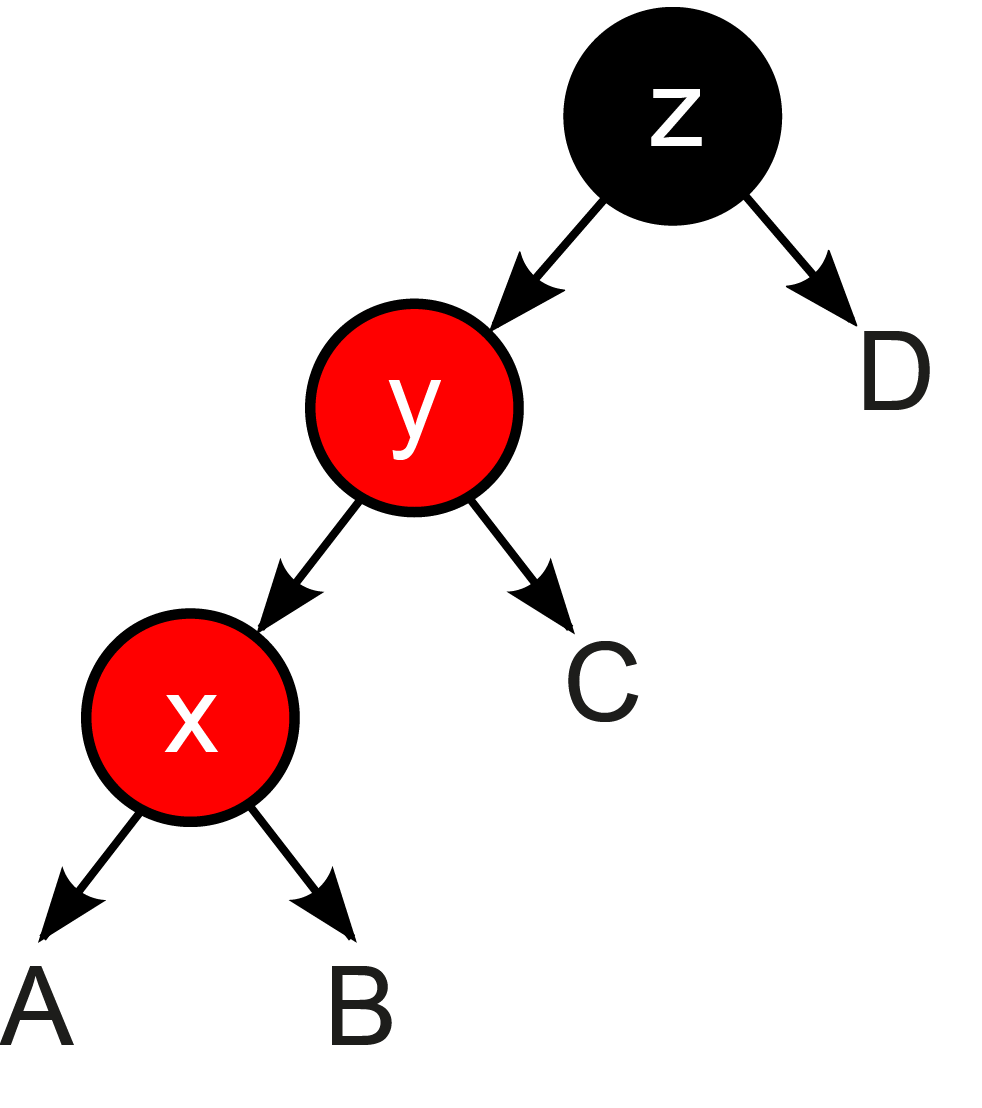
\includegraphics[width=0.8\textwidth]{img/rbtree_case_1.png}
\vspace{1cm}
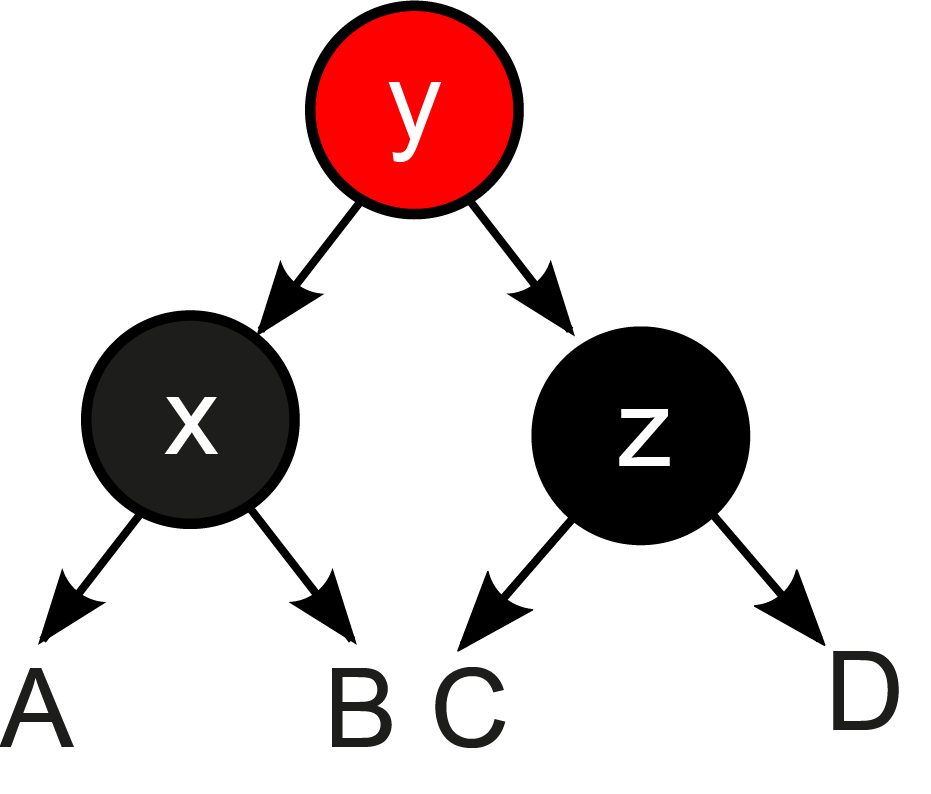
\includegraphics[width=0.8\textwidth]{img/rbtree_solution.png}
\end{columns}
\end{frame}


\begin{frame}[fragile]{Red-Black Tree in Rust}
\begin{columns}
\column{0.75\textwidth}
\begin{lstlisting}[
  language=Rust,
  caption={Tree rotation without allocation, \textit{in-place}.},
  basicstyle=\footnotesize\ttfamily
]
fn rotate_right(&mut self) {
  let self_tree = std::mem::replace(self, Empty);
  if let Node(c1, mut left, y, c) = self_tree {
    let left_tree = std::mem::replace(&mut *left, Empty);
    if let Node(c2, a, x, b) = left_tree {
      *left = Node(c1, b, y, c);
      *self = Node(c2, a, x, left);
    } else {
      *left = left_tree;
      *self = Node(c1, left, y, c);
    }
  }
}
\end{lstlisting}
\column{0.2\textwidth}
\centering
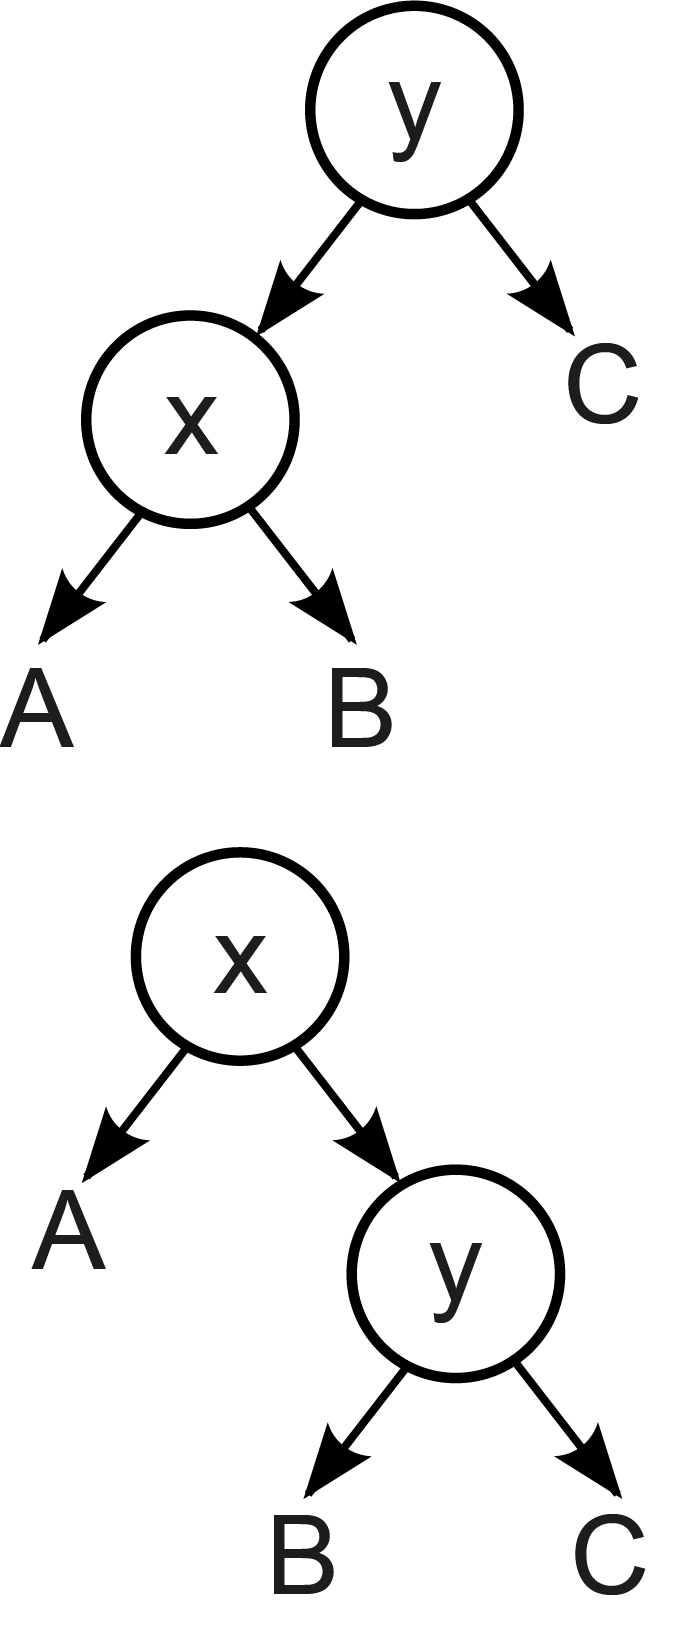
\includegraphics[width=0.8\textwidth]{img/rotate_right.png}
\end{columns}
\end{frame}


\begin{frame}[fragile]{Spin it up}
\begin{onlyenv}<1>
OK, then let's try it! \\
\begin{lstlisting}[style=short]
$ STAINLESS_FLAGS='--timeout=60' cargo stainless
\end{lstlisting}
\end{onlyenv}

\begin{onlyenv}<2>
\textbf{\alert{INVALID}}
\begin{lstlisting}[style=short]
- Result for 'postcondition' VC for balance @?:?:\\
...\\
  => INVALID\\
Found counter-example:\\
  self: MutCell[RBTree[Int]] -> ...
\end{lstlisting}
\end{onlyenv}
\end{frame}

\begin{frame}[fragile]{Red-Black Tree in Rust}
\begin{onlyenv}<1>
\begin{lstlisting}[language=Rust, caption={Pattern match acts like an \lstinline!else if!}.]
fn balance(&mut self) {
  match self {
    Node(Black, left, _, _) if left.is_red() => {
      match &mut **left {
        Node(Red, ll, _, _) if ll.is_red() => { ... }
        ...
      }
    }
    Node(Black, _, _, right) if right.is_red() => { ... }
    _ => {}
  }
}
\end{lstlisting}
\end{onlyenv}
\begin{onlyenv}<2>
\begin{lstlisting}[language=Rust, caption={Solved bug in balance function.}]
fn balance(&mut self) {
  if let Node(Black, left, _, _) = self {
    if left.is_red() {
      match &mut **left {
        Node(Red, ll, _, _) if ll.is_red() => { ... }
        ...
      }
    }
  }
  if let Node(Black, _, _, right) = self {
    if right.is_red() { ... }
  }
}
\end{lstlisting}
\end{onlyenv}
\end{frame}

\begin{frame}{Required New Features}
\begin{itemize}
\item Heap allocation
\item Methods on data types
\item Full support for mutability
\item Shared and mutable references
\item \lstinline!old! helper in postconditions
\end{itemize}
\end{frame}

\section{Tool Overview}

\begin{frame}{How it works}
\begin{itemize}
  \item Verification by Stainless in Scala
  \item \texttt{rust-stainless} is a frontend to Stainless
  \item Translate Rust fragment to Scala fragment supported by Stainless
  \item Get verification result back
\end{itemize}
\end{frame}

\begin{frame}{Pipeline}
\centering
\begin{tikzpicture}[
  rect/.style={
    rectangle,
    minimum height=8mm,
    text centered,
    draw=black
  },
  align=center,
  node distance=1.1cm,
  auto
]
\node (rustc)     []   {\texttt{rustc}};
\node (tool)      [right= 2cm of rustc]   {Rust-Stainless};
\node (stainless) [right= 2.5cm of tool]   {Stainless (JVM)};

\node (source)  [rect, below= 0.2cm of rustc] {Source};
\node (ast)     [rect, below of=source] {AST};
\node (hir)     [rect, below of=ast] {HIR};
\node (thir)    [rect, below of=hir] {THIR};
\node (mir)     [rect, below of=thir] {MIR};
\node (llvm)    [rect, below of=mir,  draw=gray, text=gray] {LLVM-IR};
\node (asm)     [rect, below of=llvm, draw=gray, text=gray] {ASM (Target)};

\node (srast)   [rect, below= 0.2cm of tool] {Stainless AST (Rust)};
\node (binary)  [rect, below of=srast] {Binary};
\node (rvr)     [rect, right=of thir] {Verification Result (Rust)};

\node (ssast)   [rect, below= 0.2cm of stainless] {Stainless AST (Scala)};
\node (svr)     [rect, below of=ssast] {Verification Result (Scala)};
\node (json)    [rect, below of=svr] {JSON};

% down arrows
\draw[->] (source) -- (ast);
\draw[->] (ast) -- (hir);
\draw[->] (hir) -- (thir);
\draw[->] (thir) -- (mir);
\draw[->, draw=gray] (mir) -- (llvm);
\draw[->, draw=gray] (llvm) -- (asm);
\draw[->] (srast) -- (binary);
\draw[->] (ssast) -- (svr);
\draw[->] (svr) -- (json);

\draw[->] (hir.east) to    [out=0, in=180] (srast.west);
\draw[->] (thir.east) to   [out=0, in=180] (srast.west);
\draw[->] (binary.east) to [out=0, in=180] (ssast.west);
\draw[->] (json.south) to  [out=270, in=0] (rvr.east);
\end{tikzpicture}

\end{frame}




\section{Mutability Translation}

\begin{frame}{Goal}
Translate Rust mutability and references to Scala while providing runtime
equivalence in Scala and verification in Stainless.
\end{frame}

\begin{frame}{Challenges}
\begin{itemize}
\item Explicit references (borrows) and ownership in Rust don't exist in Scala.
\item Heap- \& stack-allocated data in Rust vs everything on the heap in Scala.
\end{itemize}
\end{frame}


\begin{frame}[fragile]{Mutable Cells}
To make references possible, a layer of indirection is needed. All mutability is
modelled with the mutable cell object:
\begin{lstlisting}[language=Scala, style=short]
case class MutCell[T](var value: t)
\end{lstlisting}
\vfill
\begin{block}{Idea}
Whenever something is (possibly) mutable, we wrap it into a mutable cell.
\end{block}
\vfill
In Scala (on the JVM):
\begin{itemize}
  \item all objects are on the heap,
  \item objects are handled by reference only.
\end{itemize}
\end{frame}

\begin{frame}[fragile]{Example}
This allows modelling references by wrapping values in mutable cells:

\begin{columns}
\column{0.35\textwidth}
\begin{lstlisting}[language=Rust]
struct A<T> {
  a: T, b: i32
}
let x = A {
  a: "foo", b: 123
}
let mut y = 123;
assert!(y == x.b);
\end{lstlisting}
\column{0.6\textwidth}
\begin{lstlisting}[language=Scala]
case class A[T](
  a: MutCell[T], b: MutCell[Int]
)
val x = MutCell(
  A(MutCell("foo"), MutCell(123))
)
val y = MutCell(123)
assert(y.value == x.value.b.value)
\end{lstlisting}
\end{columns}

A reference to \lstinline!y! in Rust, e.g. \lstinline!&mut y!, is now equivalent
to the mutable cell \lstinline!y! in Scala.
\end{frame}



\begin{frame}{Ownership and Aliasing}
To model Rust's ownership type system, the translation uses the
\lstinline!freshCopy! operator of Stainless.

\begin{itemize}
\item Semantically, a deep copy
\item Models move and copy semantics
\item Helps avoid aliasing restrictions of the Stainless imperative phase
\end{itemize}
\end{frame}

\begin{frame}[fragile]{Example}
\begin{columns}[T]
\column{.4\textwidth}
\begin{lstlisting}[language=Rust]
let x = (
  123,
  false
);
// copies `x`
let mut y = x;

y.0 = 456;
// holds:
assert!(x.0 == 123)
\end{lstlisting}
\column{.6\textwidth}
\begin{onlyenv}<1>
\begin{lstlisting}[language=Scala]
val x = MutCell(Tuple2(
  MutCell(123),
  MutCell(false)
))
// shares tuple object `x.value`
val y = MutCell(x.value)
// i.e. x.value == y.value
y.value._0.value = 456
// fails:
assert(x.value._0.value == 123)
\end{lstlisting}
\end{onlyenv}
\begin{onlyenv}<2>
\begin{lstlisting}[language=Scala]
val x = MutCell(Tuple2(
  MutCell(123),
  MutCell(false)
))
// copies tuple object `x.value`
val y = MutCell(freshCopy(x.value))
// i.e. x.value != y.value
y.value._0.value = 456
// holds:
assert(x.value._0.value == 123)
\end{lstlisting}
\end{onlyenv}
\end{columns}
\only<2>{Insert \lstinline!freshCopy! wherever data is moved or copied.}
\end{frame}

\begin{frame}[fragile]{Memory Replace}
\begin{columns}[T]
\column{.42\textwidth}
\begin{lstlisting}[language=Rust]
fn f(a: &mut A) -> A {
  std::mem::replace(
    a,
    A { a: "bar", b: 0 }
  )
}
\end{lstlisting}
\column{.55\textwidth}
\begin{lstlisting}[language=Scala]
def f(a: MutCell[A]): A = {
  val res = freshCopy(a.value)
  a.value = A(
    MutCell("bar"), MutCell(0)
  )
  freshCopy(res)
}
\end{lstlisting}
\end{columns}
\end{frame}


\section{Conclusions}

\subsection{Result}

\begin{frame}{Result}
\begin{itemize}
  \item \texttt{rust-stainless} tool supports a large part of Rust
  \item Full support for mutable and shared references
  \item Frontend only accounts for 5~\% of running time
\end{itemize}
\end{frame}

\begin{frame}{Added Features}
Other than mutability, this project added:
\begin{itemize}
\item Implementation blocks, traits and laws (algebraic properties),
\item Stainless Map and Set implementation,
\item \lstinline!return! keyword,
\item Pattern matching for tuples,
\item and many notational improvements.
\end{itemize}
\end{frame}

\subsection{Limitations}

\begin{frame}[fragile]{Limitations}
\begin{itemize}
\item Missing Rust features: arrays, loops, iterators and closures
\item One-crate-limitation
\item No access to lifetimes
\item Refinement lifting in the backend
\item Stainless aliasing restrictions
\end{itemize}
\end{frame}

\subsection{Future Work}

\begin{frame}{Future Work}
\begin{itemize}
  \item Solving the \textbf{one-crate-limitation} by allowing specifications
  for crate-external items.

  \item Using the new fully imperative phase of Stainless currently in
  development to overcome aliasing restrictions.

  \item Providing Rust counter-examples.

  \item Uncover new use-cases, for example in the blockchain context.
\end{itemize}
\end{frame}

\begin{frame}{That was}
\centering
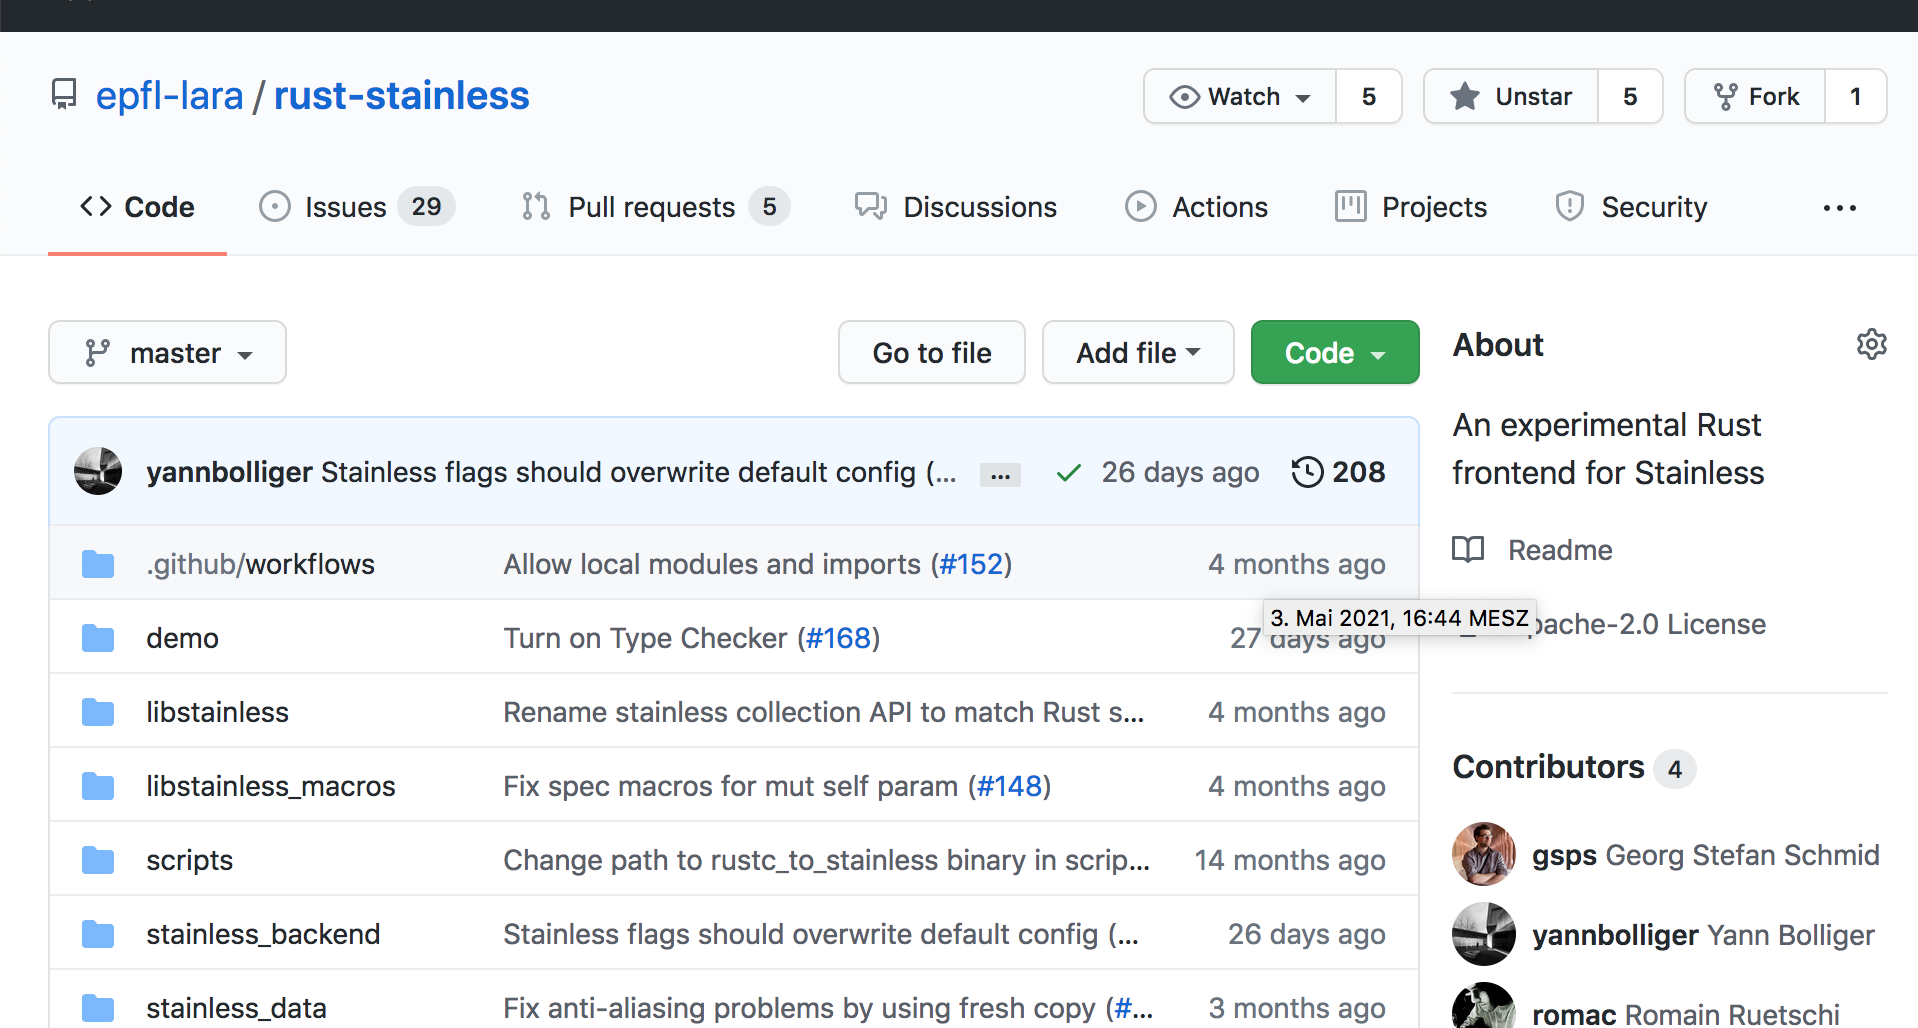
\includegraphics[width=0.9\textwidth]{img/github.png}
\end{frame}

\begin{frame}[standout]
Thank you!
\end{frame}

\begin{frame}[standout]
Questions?
\end{frame}


\begin{frame}[allowframebreaks]{References}
  \bibliography{bib}
  \bibliographystyle{IEEEtranS}
\end{frame}


\appendix

\begin{frame}[fragile]{Red-Black Tree in Rust}
\begin{lstlisting}[language=Rust, caption={Insert method}]
impl RBTree<i32> {
  pub fn insert(&mut self, t: i32) {
    // Insert and color the root black.
    self.ins(t);
    if let Node(ref mut c, _, _, _) = self {
      *c = Black;
    }
  }
}
\end{lstlisting}
\end{frame}

\begin{frame}[fragile]{Implementation blocks, traits and laws}
\begin{onlyenv}<1>
\begin{lstlisting}[
  language=Rust,  basicstyle=\footnotesize\ttfamily,
]
trait Equals {
  fn equals(&self, x: &Self) -> bool;
  fn not_equals(&self, x: &Self) -> bool {
    !self.equals(x)
  }
  #[law]
  fn reflexive(x: &Self) -> bool {
    x.equals(x)
  }
  #[law]
  fn symmetric(x: &Self, y: &Self) -> bool {
    x.equals(y) == y.equals(x)
  }
  #[law]
  fn transitive(x: &Self, y: &Self, z: &Self) -> bool {
    !(x.equals(y) && y.equals(z)) || x.equals(z)
  }
}
\end{lstlisting}
\end{onlyenv}
\begin{onlyenv}<2>
\begin{lstlisting}[
  language=Rust,
  basicstyle=\footnotesize\ttfamily,
]
impl Equals for i32 {
  fn equals(&self, y: &i32) -> bool {
    *self == *y
  }
}
enum List<T> {
  Nil,
  Cons(T, Box<List<T>>)
}
impl<T: Equals> Equals for List<T> {
  fn equals(&self, other: &List<T>) -> bool {
    match (self, other) {
      (List::Nil, List::Nil) => true,
      (List::Cons(x, xs), List::Cons(y, ys)) => x.equals(y) && xs.equals(ys),
      _ => false,
    }
  }
  ...
}
\end{lstlisting}
\end{onlyenv}
\begin{onlyenv}<3>
\begin{lstlisting}[language=Scala, basicstyle=\footnotesize\ttfamily]
abstract class Equals[Self] {
  def equals(self: Self, x: Self): Boolean
  def notEquals(self: Self, x: Self): Boolean = !this.equals(self, x)
  @law def reflexive(x: Self): Boolean = this.equals(x, x)
  ...
}
case object i32asEquals extends Equals[Int] {
  def equals(self: Int, y: Int): Boolean = self == y
}
case class ListasEquals[T](ev0: Equals[T]) extends Equals[List[T]] {
  def equals(self: List[T], other: List[T]): Boolean =
    (self, other) match {
      case (Nil(), Nil()) => true
      case (Cons(x,xs),Cons(y,ys)) => ev0.equals(x,y) && this.equals(xs,ys)
      case _ => false
    }
  ...
}
val list = Cons(123, Nil())
ListasEquals[i32](i32asEquals).equals(list, Nil())
\end{lstlisting}
\end{onlyenv}
\end{frame}

\begin{frame}{Heap Allocation}
With mutable cells and memory safety, heap allocation is for free:
\begin{itemize}
  \item Achieved with Boxes in Rust, otherwise data is stack-allocated.
  \item Distinction not needed in Scala because all objects are on the heap.
  \item Translation erases boxes because it wraps the variables in mutable
  cells anyway.
\end{itemize}
\end{frame}

\begin{frame}[fragile]{Aliasing Limitations}
\begin{columns}[T]
\column{.35\textwidth}
\begin{lstlisting}[
  language=Rust
]
let mut a = 123;
let mut b = 456;
let mut x = &mut a;

x = &mut b;
\end{lstlisting}

\column{.65\textwidth}
\begin{lstlisting}[
  language=Scala
]
val a: MutCell[Int] = MutCell[Int](123)
val b: MutCell[Int] = MutCell[Int](456)
val x: MutCell[MutCell[Int]] =
  MutCell[MutCell[Int]](a)
x.value = b // Illegal aliasing
\end{lstlisting}
\end{columns}
\end{frame}
